\chapter{Our solution} \label{our:solution}


% uvod, co je v kapitole, nejdriv...
% obecne algorithmus bez rozzepsaneho gpcka

% Prvni cats - GPcko (zakodovani, init, operat., fitness jak se pocita (ale vic dole),...
% Druha - Sklearn strana, eval, samples,...

% Posledni- implementace, deap,...

% experimenty 4

In our solution we design an AutoML system for workflow optimization based on
developmental genetic programming. Compared to existing systems it supports 
arbitrary-sized pipelines as well as complex ensemble structures. We first
present in what way we use the genetic programming, then we describe the
pipeline evaluation process.

\section{Evolutionary optimization of pipelines}
The algorithm corresponds to the schema of a general genetic algorithm
\ref{alg:EA}. In this section we describe the necessary components of the
algorithm.

\subsection{Individual encoding}
The individual encoding is one of the most important parts of this system. With
ensembles and complex feature preprocessing methods like stacking or feature
union, most of the pipelines become in fact directed acyclic graphs (figure 
\ref{pic02:pipeline}). Therefore, we cannot directly use the simple tree-based
encoding. Instead we use the developmental GP with cellular encoding described
in section \ref{devGP}.
\begin{figure}[ht]\centering
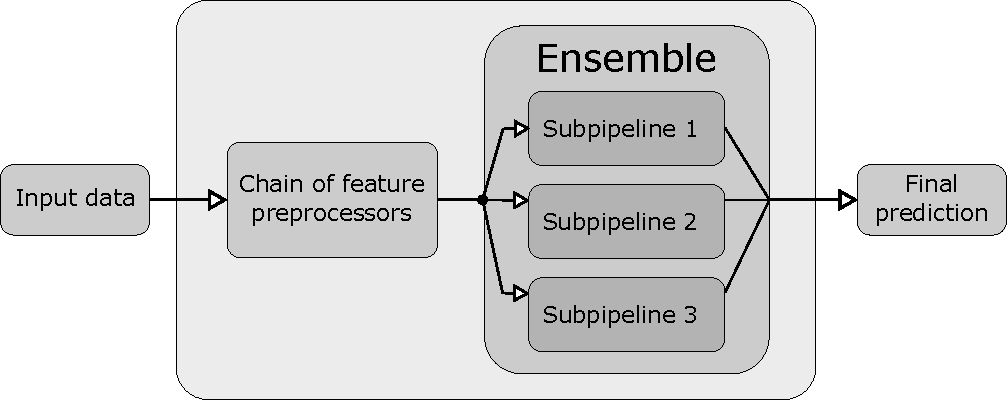
\includegraphics[width=0.8\textwidth]{../img/pipeline-pdfa.pdf}
\caption{Schema of an example pipeline}
\label{pic02:pipeline}
\end{figure}

In our case, the cell is an empty pipeline. To create a complex pipeline, we
modify it by inserting steps into it. To demonstrate the process, 
\begin{figure}[h]\centering
    \subfloat[label 1]{{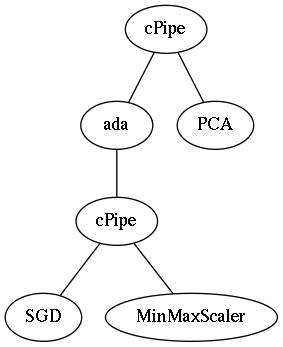
\includegraphics[width=0.5\textwidth]{../img/ada.png} }}%
    \qquad
    \subfloat[label 2]{{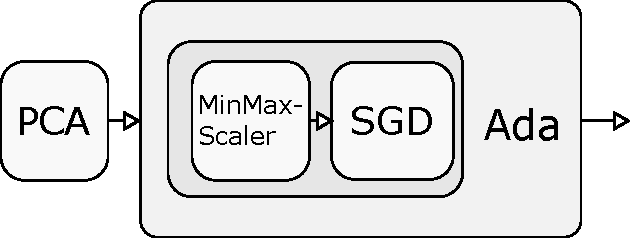
\includegraphics[width=0.5\textwidth]{../img/ada-pdfa.pdf} }}%
    \caption{2 Figures side by side}%
    \label{fig:example}%
\end{figure}

\subsection{Genetic operators}

\subsection{Fitness and selection}

\section{Evaluation and performance estimation}

\section{Implementation}